Una família vol comprar un terreny per a fer-s'hi una casa envoltada de penya-segats amb vistes al mar. En
aquella zona de la costa, els penya-segats segueixen les rectes $y=0$ i $y=3x$. A més, la família vol que el
terreny sigui triangular i que el tercer costat del triangle passi pel punt $P=(1,1)$, tal com es pot veure en
la figura.
\begin{center}
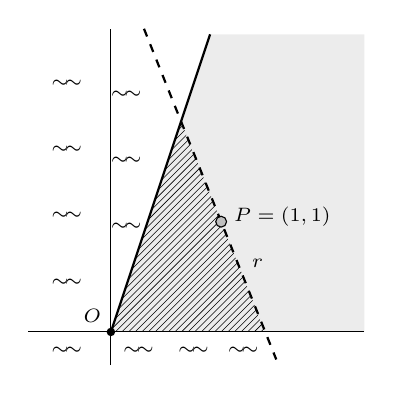
\begin{tikzpicture}[scale=1.4]
  \fill[gray!15] (0,0) -- (0.9,2.7) -- (2.3,2.7) -- (2.3,0) -- cycle;
  \begin{scope}
    \clip (0,0) -- (0.6364,1.9091) -- (1.4,0) -- cycle;
    \foreach \t in {-2,-1.94,...,1.5} \draw[very thin] (\t,0) -- ++(2.2,2.2);
  \end{scope}
  \draw[thin] (-0.75,0) -- (2.3,0);
  \draw[thin] (0,-0.3) -- (0,2.75);
  \draw[thick] (0,0) -- (0.9,2.7);
  \draw[thick,dashed] (0.3,2.75) -- (1.5,-0.25);
  \fill (0,0) circle (1.1pt);
  \node[above left,font=\scriptsize] at (0,0) {$O$};
  \draw[fill=gray!50] (1,1) circle (1.4pt);
  \node[right,font=\scriptsize] at (1.03,1.05) {$P=(1,1)$};
  \node[font=\scriptsize] at (1.33,0.62) {$r$};
  \foreach \p in {(-0.4,0.45),(-0.4,1.05),(-0.4,1.65),(-0.4,2.25),(0.14,0.95),(0.14,1.55),(0.14,2.15),
                  (-0.4,-0.17),(0.25,-0.17),(0.75,-0.17),(1.2,-0.17)}
    \node[font=\scriptsize] at \p {$\sim\!\sim$};
\end{tikzpicture}
\end{center}

\begin{apartats}

\apartat{1}
Plantegeu l'equació de la recta $r$ que defineix el tercer costat del triangle en funció del seu pendent $m$,
i comproveu que l'àrea del terreny ve donada per $A(m)=\dfrac32\cdot\dfrac{m^2-2m+1}{m^2-3m}$.

\begin{solucio}
Tenint en compte que la recta $r$ ha de passar pel punt $P=(1,1)$ i que $m$ és el seu pendent, la recta $r$ té
per equació $y-1=m(x-1)$. La mida de la base del triangle és l'abscissa del punt d'intersecció de la recta $r$
amb l'eix $OX$:
\[
\left.\begin{aligned}y-1&=m(x-1)\\y&=0\end{aligned}\right\}\;\rightarrow\;0-1=m(x-1)\;\rightarrow\;x=\frac{m-1}{m}.
\]
I l'alçada del triangle és l'ordenada del punt d'intersecció de la recta $r$ amb $y=3x$:
\[
\left.\begin{aligned}y-1&=m(x-1)\\y&=3x\end{aligned}\right\}\;\rightarrow\;3x-1=m(x-1)\;\rightarrow\;
x=\frac{m-1}{m-3},\quad y=3\cdot\frac{m-1}{m-3}.
\]
La funció a minimitzar és la que calcula l'àrea del triangle:
\[
A(m)=\frac12\cdot\frac{m-1}{m}\cdot3\cdot\frac{m-1}{m-3}=\frac32\cdot\frac{m^2-2m+1}{m^2-3m}.
\]
Parlant estrictament, el valor de l'àrea és $A(m)=\left|\frac32\cdot\frac{m^2-2m+1}{m^2-3m}\right|$, perquè hi
ha valors de $m$ per als quals aquesta expressió és negativa. No ho tingueu en compte si s'ignora aquest
detall.

\textit{Pauta oficial:} 0,25 per l'equació del feix de rectes; 0,25 per la mida de la base del triangle; 0,25
per l'alçada, i 0,25 pel càlcul final de l'àrea (tot en funció de $m$).
\end{solucio}

\apartat{1,5}
Calculeu el valor de $m$ que fa que l'àrea d'aquest terreny (i, per tant, el seu preu) sigui mínima. Quin és el
valor d'aquesta àrea?

\begin{solucio}
Derivem la funció àrea i igualem a zero per trobar els possibles extrems relatius:
\[
A'(m)=\frac32\cdot\frac{(2m-2)\left(m^2-3m\right)-\left(m^2-2m+1\right)(2m-3)}{\left(m^2-3m\right)^2}
=\frac32\cdot\frac{-m^2-2m+3}{\left(m^2-3m\right)^2}=0,
\]
\[
-m^2-2m+3=0\;\rightarrow\;m=\frac{2\pm\sqrt{4-4(-1)3}}{-2}=\frac{2\pm4}{-2}=1,\ -3 .
\]
Per comprovar si són màxims o mínims, fem la segona derivada:
\[
A''(m)=\frac32\cdot\frac{(-2m-2)\left(m^2-3m\right)^2-\left(-m^2-2m+3\right)2\left(m^2-3m\right)(2m-3)}{\left(m^2-3m\right)^4},
\]
i, com que $A''(-3)=\frac1{54}>0$ i $A''(1)=-\frac32<0$, el mínim correspon a $m=-3$ (segons l'esbós, el
pendent ja ha de ser negatiu).\\
Alternativament, podem estudiar el creixement i decreixement de la funció $A(m)$. Aquests venen donats pel
signe de la primera derivada, però, com que aquesta té un quadrat al denominador, dependrà només del signe
del numerador, $-m^2-2m+3$. Això és una paràbola oberta cap avall que talla l'eix $OX$ en els punts
$(-3,0)$ i $(1,0)$; així doncs, per a $m<-3$ la derivada és negativa i la funció decreix, i per a $-3<m<1$
la derivada és positiva i la funció creix, per la qual cosa en $m=-3$ l'àrea és mínima. El valor d'aquesta
àrea és
\[
A(-3)=\frac32\cdot\frac{(-3)^2-2(-3)+1}{(-3)^2-3(-3)}=\frac32\cdot\frac{16}{18}=\frac43\ \text{u}^2 .
\]

\textit{Pauta oficial:} 0,5 per la derivada; 0,25 per calcular els punts crítics; 0,5 per justificar el mínim,
i 0,25 per calcular el valor de l'àrea.
\end{solucio}

\end{apartats}
